% Relatório AP2 - Rivalidade no mercado de carros elétricos no Brasil
% Overleaf: suba este arquivo e a pasta figuras e compile com pdfLaTeX.
\documentclass[10pt,a4paper]{article}
\usepackage[utf8]{inputenc}
\usepackage[T1]{fontenc}
\usepackage[brazil]{babel}
\usepackage{lmodern}
\usepackage[a4paper,margin=1.8cm]{geometry}
\usepackage{graphicx}
\usepackage{booktabs}
\usepackage{enumitem}
\usepackage{microtype}
\usepackage[hidelinks]{hyperref}
\setlist{nosep,leftmargin=*}
\setlength{\parskip}{3pt}
\setlength{\parindent}{0pt}
\usepackage{titlesec}
\titlespacing*{\section}{0pt}{6pt}{2pt}
\titleformat*{\section}{\normalsize\bfseries}

\begin{document}

\begin{center}
{\Large\bfseries Rivalidade no mercado de carros elétricos no Brasil (2020--2026)}\\[3pt]
Relatório do projeto --- AP2 \quad$\cdot$\quad Ibmec\\[2pt]
\small Integrantes: Nome 1, Nome 2, Nome 3, Nome 4
\end{center}

\section{Objetivo e setor escolhido}
Escolhemos o mercado de \textbf{carros 100\% elétricos (BEV)}, um setor que em seis anos saiu de algumas centenas de unidades para quase 190 mil, teve a entrada agressiva de montadoras chinesas e mudanças de política tributária. O objetivo foi medir o nível de rivalidade entre as marcas e explicar o que o mudou, entregando as análises num \textbf{portal interativo} em que o usuário escolhe o ano, as marcas e os painéis que quer ver.

\section{Dados e fontes}
Todos os dados são públicos e coletados por script (\texttt{coleta\_dados.py}); cada linha tem uma coluna \texttt{status} que separa o dado oficial do estimado.
\begin{itemize}
  \item \textbf{Fenabrave} --- informativos mensais de emplacamento (jan/2024 a out/2026): ranking das 15 maiores marcas de elétricos, de híbridos e de todos os automóveis. É a base principal.
  \item \textbf{ABVE} --- totais anuais de 2020 a 2023. A divisão por marca nesses anos é \textbf{estimativa do grupo}, pois a Fenabrave não publicava o ranking de elétricos.
  \item \textbf{Comex Stat (MDIC)} --- importações da NCM 8703.80.00 (veículos só elétricos) por país, em unidades e US\$.
  \item \textbf{Banco Central (SGS)} --- juros de financiamento de veículos, Selic, IPCA e câmbio.
  \item \textbf{Tabela FIPE} --- preço do zero km de cada modelo elétrico, mês a mês.
  \item \textbf{Receita Federal/imprensa} --- alíquotas do imposto de importação (0\% em 2023; 10\%, 18\%, 25\% e 35\% em jul/2026), lançamentos e fichas técnicas.
\end{itemize}

\section{Variáveis e método}
A rivalidade foi medida por indicadores clássicos de organização industrial: \textbf{participação de mercado}; \textbf{HHI} (soma dos quadrados das participações; abaixo de 1.500 é baixa concentração, acima de 2.500 é alta, critério do CADE); \textbf{CR1} e \textbf{CR4}; \textbf{número de empresas equivalentes} (10.000/HHI); \textbf{entrada de novas marcas}; e \textbf{instabilidade de participação} (Hymer-Pashigian: pontos percentuais do mercado que trocam de mãos de um ano para o outro). Para preços e barreiras usamos a FIPE corrigida pelo IPCA e as alíquotas de importação. Tudo foi feito em Python (pandas, statsmodels, scikit-learn).

\section{Análise principal: concentração ao longo do tempo}
\begin{minipage}[t]{0.52\linewidth}\vspace{0pt}
\centering\footnotesize\setlength{\tabcolsep}{4pt}
\begin{tabular}{@{}lrrrrr@{}}
\toprule
Ano & Carros & HHI & Líder (CR1) & CR4 & Equiv. \\
\midrule
2020$^*$ & 801    & 1.842 & Nissan 29\% & 80\% & 5,4 \\
2021$^*$ & 2.851  & 1.250 & Porsche 18\% & 61\% & 8,0 \\
2022$^*$ & 8.460  & 1.516 & Volvo 32\% & 61\% & 6,6 \\
2023$^*$ & 19.310 & 3.343 & BYD 53\% & 85\% & 3,0 \\
2024 & 60.174  & 5.478 & BYD 73\% & 93\% & 1,8 \\
2025 & 79.415  & 5.274 & BYD 72\% & 87\% & 1,9 \\
2026$^\dagger$ & 186.514 & 4.353 & BYD 63\% & 90\% & 2,3 \\
\bottomrule
\end{tabular}\\[2pt]
\footnotesize $^*$ divisão por marca estimada. $^\dagger$ jan--out.
\end{minipage}\hfill
\begin{minipage}[t]{0.45\linewidth}\vspace{0pt}
\centering
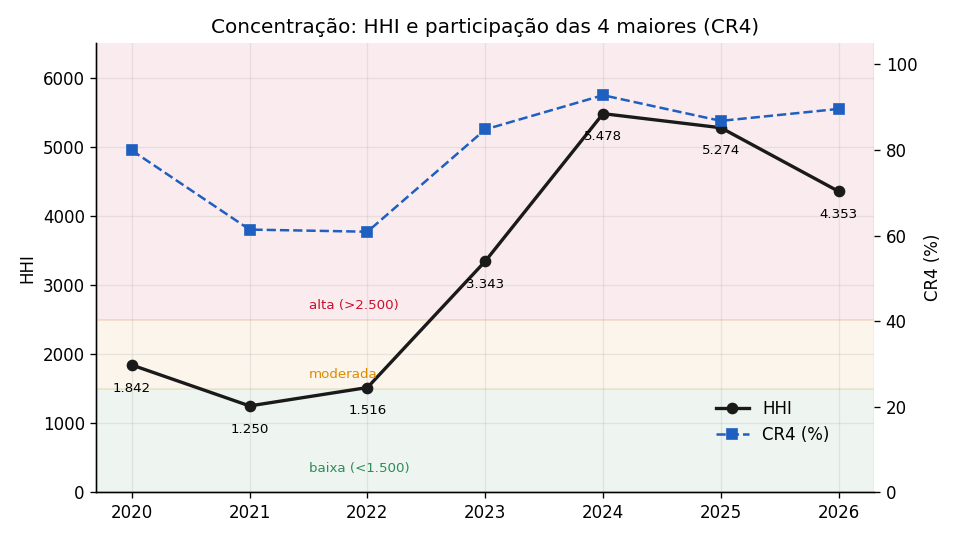
\includegraphics[width=\linewidth]{figuras/03_hhi_cr4.png}
\end{minipage}

\smallskip
O setor passou por três fases. \textbf{Até 2022}, um nicho pequeno e disputado por marcas premium importadas (Volvo, BMW, Porsche, Audi, Mercedes, com mais da metade do mercado), com concentração baixa a moderada. \textbf{Em 2023--2025}, a BYD entrou com carros abaixo de R\$\,150 mil, ficou com mais de 70\% do mercado e o HHI passou de 5.000, equivalente a menos de duas empresas do mesmo tamanho. \textbf{Em 2026}, a Geely (EX2) virou a segunda força com 18\% e o HHI caiu para 4.353: a concentração ainda é alta, mas a rivalidade aumentou. As premium caíram para cerca de 2\%.

\section{Análises complementares}
\begin{itemize}
  \item \textbf{Definição de mercado.} Em 2026 o HHI é 4.553 só entre elétricos, 2.020 incluindo híbridos e 916 entre todos os automóveis (BYD com 64\%, 40\% e 10\%). O ``quase monopólio'' só vale na definição mais estreita.
  \item \textbf{Robustez.} Uma simulação de Monte Carlo com erro de até 30\% nas estimativas de 2020--2023 mostra que a faixa de 2022 é incerta, mas a virada de 2023 para concentração alta não depende das estimativas.
  \item \textbf{O que mexeu na liderança.} Numa série temporal interrompida com dados mensais, a chegada do Geely EX2 em volume (nov/2025) está associada a $-10$ p.p. na participação da BYD ($p=0{,}001$); as altas do imposto não tiveram efeito significativo isolado.
  \item \textbf{Imposto e estoque.} Antes de cada alta do imposto as importações disparam e depois caem de 4 a 7 vezes: as marcas antecipam estoque. 97\% dos elétricos importados desde 2024 vêm da China.
  \item \textbf{Preços.} Na FIPE, o elétrico mais barato caiu de R\$\,157 mil para R\$\,101 mil (valores reais, 2024--2026), e os modelos abaixo de R\$\,150 mil foram de 0 para 12. Numa regressão hedônica ($R^2=0{,}87$), com a mesma potência e bateria uma marca chinesa custa 26\% menos.
  \item \textbf{Grupos estratégicos.} Um agrupamento k-means separa três faixas: entrada (\textasciitilde R\$\,125 mil), intermediária (\textasciitilde R\$\,232 mil) e premium (\textasciitilde R\$\,543 mil); a rivalidade por preço está concentrada nas duas primeiras.
\end{itemize}

\section{O portal}
O portal (\texttt{portal/index.html}) tem três abas. \textbf{Dados e concentração}: indicadores do ano escolhido, participação por marca, HHI e CR4, ranking, comparação com outros setores, preços e linha do tempo; o usuário liga e desliga painéis e marcas, e um \textbf{simulador} recalcula o HHI se uma marca ganhar participação de outra ou se duas se fundirem. \textbf{Análise estratégica}: 5 Forças de Porter ajustáveis, estratégias genéricas, Mintzberg, Chandler, SWOT e modelo TAM. \textbf{Série mensal e estatística}: os resultados das análises complementares. Os dados e o resumo podem ser copiados para compartilhar.

\section{Conclusões}
A rivalidade no mercado de elétricos é \textbf{alta em preço, mas com estrutura muito concentrada}. A BYD ganhou o mercado com liderança em custo, e o principal fator que reduziu sua participação foi a entrada de outra chinesa com preço parecido, não a política tributária. O imposto de 35\% funciona como barreira de entrada para quem só importa e favorece quem monta no Brasil (BYD em Camaçari). Para as empresas, o desafio é sustentar margem numa guerra de preços enquanto o mercado ainda dobra a cada ano; a oportunidade está na produção local e nas faixas de preço intermediárias.

\textbf{Limitações:} a divisão por marca de 2020--2023 é estimada; a Fenabrave publica só as 15 maiores marcas por mês; 2026 vai até outubro.

\end{document}
